\documentclass{mwrep}
\usepackage{graphicx}
\usepackage[space]{grffile}
% Polskie znaki
\usepackage{polski}
\usepackage[utf8]{inputenc}
\usepackage[T1]{fontenc}
\usepackage{lmodern}
\usepackage{indentfirst}

% Strona tytułowa
\usepackage{pgfplots}
\usepackage{siunitx}
\usepackage{paracol}
\usepackage{gensymb}

% Pływające obrazki
\usepackage{float}
\usepackage{svg}
\usepackage{graphicx}

% table of contents refs
\usepackage{hyperref}
\usepackage{cleveref}
\usepackage{booktabs}
\usepackage{listings}
\usepackage{placeins}
\usepackage{xcolor}
\usepackage[left= 3cm, textwidth=10cm]{geometry}
\usepackage{epstopdf}
\epstopdfsetup{outdir=./}

\sisetup{detect-weight,exponent-product=\cdot,output-decimal-marker={,},per-mode=symbol,binary-units=true,range-phrase={-},range-units=single}
\SendSettingsToPgf
%konfiguracje pakietu listings
\lstset{
	backgroundcolor=\color{gray},
	frame=single,
	breaklines=true,
}
\lstdefinestyle{customlatex}{
	basicstyle=\footnotesize\ttfamily,
	%basicstyle=\small\ttfamily,
}
\lstdefinestyle{customc}{
	breaklines=true,
	frame=tb,
	language=C,
	xleftmargin=0pt,
	showstringspaces=false,
	basicstyle=\small\ttfamily,
	keywordstyle=\bfseries\color{green!40!black},
	commentstyle=\itshape\color{purple!40!black},
	identifierstyle=\color{blue},
	stringstyle=\color{orange},
}
\lstdefinestyle{custommatlab}{
	captionpos=t,
	breaklines=true,
	frame=tb,
	xleftmargin=0pt,
	language=matlab,
	showstringspaces=false,
	%basicstyle=\footnotesize\ttfamily,
	basicstyle=\scriptsize\ttfamily,
	keywordstyle=\bfseries\color{green!40!black},
	commentstyle=\itshape\color{purple!40!black},
	identifierstyle=\color{blue},
	stringstyle=\color{orange},
}

%wymiar tekstu 
\textwidth 160mm \textheight 247mm

%ustawienia pakietu pgfplots
\pgfplotsset{
tick label style={font=\scriptsize},
label style={font=\small},
legend style={font=\small},
title style={font=\small}
}

\def\figurename{Rys.}
\def\tablename{Tab.}

%konfiguracja liczby 
\setcounter{topnumber}{0}%2
\setcounter{bottomnumber}{3}%1
\setcounter{totalnumber}{5}%3
\renewcommand{\textfraction}{0.01}%0.2
\renewcommand{\topfraction}{0.95}%0.7
\renewcommand{\bottomfraction}{0.95}%0.3
\renewcommand{\floatpagefraction}{0.35}%0.5

\begin{document}
\frenchspacing
\pagestyle{uheadings}

%strona 
\title{\bf Sprawozdanie z projektu i ćwiczenia laboratoryjnego nr 3, zadanie nr 4\vskip 0.1cm}
\author{Piotr Chachuła, Cezary Dudkiewicz, Piotr Roszkowski}
\date{2019}

\makeatletter
\renewcommand{\maketitle}{\begin{titlepage}
\begin{center}{\LARGE {\bf
Wydział Elektroniki i Technik Informacyjnych}}\\
\vspace{0.4cm}
{\LARGE {\bf Politechnika Warszawska}}\\
\vspace{0.3cm}
\end{center}
\vspace{5cm}
\begin{center}
{\bf \LARGE Projektowanie układów sterowania\\ (projekt grupowy) \vskip 0.1cm}
\end{center}
\vspace{1cm}
\begin{center}
{\bf \LARGE \@title}
\end{center}
\vspace{2cm}
\begin{center}
{\bf \Large \@author \par}
\end{center}
\vspace*{\stretch{6}}
\begin{center}
\bf{\large{Warszawa, \@date\vskip 0.1cm}}
\end{center}
\end{titlepage}
}
\makeatother

\maketitle

\tableofcontents
\part{Projekt}
\label{PROJEKT}
\chapter{Weryfikacja punktu pracy}
\label{zad1}

\section{Opis postępowania}
\label{zad1_opis}
W celu sprawdzenia poprawności punktu pracy pobudzono obiekt sterowaniem
o wartości $u = \num{0.0}$ i sprawdzeniu czy stabilizuje się on w punkcjie pracy  $y = \num{0.0}$. Do symulacji wyjscia obiektu użyto udostępnionej funkcji 
\verb+symulacja_obiektu4y.+ Do testów napisano skrypt \verb+Zad1.m. + Wyniki przedstawiono poniżej.

\section{Wyniki}
\label{zad1_wyniki}
Zgodnie z przewidywaniami wyjscie obiektu ustaliło się na wartości $y= \num{0.0}$. Punkt pracy ustalony jest więc poprawnie.
\begin{figure}[tb]
	\centering
	\includegraphics[scale=1]{Rys/punkt_pracy.eps}
	\caption{Odpowiedź obiektu na sterowania $u=\num{0.0}$}
\end{figure}

\part{Laboratoria}
\chapter {Pomiar w punkcie pracy}
\label{zad1l}

\section{Komunikacja z obiektem}

Komunikacja z obiektem odobywa się za pomocą funkcji napisanych w środowisku MatLab. Najprostszy program użyty w tym projekcie, który posłużył także do późniejszego pobierania odpowiedzi skokowych znajduje się poniżej (jest to fragment skryptu \verb|L3_1.m|).


%\begin{lstlisting}[style=custommatlab,frame=single]
\begin{lstlisting}[style=custommatlab]


    addpath('F:\SerialCommunication'); % add a path to the functions
    initSerialControl COM3 % initialise com port
   
    N = 420;
    step_response = zeros(N+1,1);
    i = 0;
    
    while(i<=N)
        %% obtaining measurements
        measurements = readMeasurements(1:7); % read measurements from 1 to 1
        
        %% processing of the measurements and new control values calculation
        disp([measurements(1),i]);
        step_response(i+1)=measurements(1);
        
        %% sending new values of control signals
        sendNonlinearControls(29)  % new corresponding control valuesdisp(measurements); % process measurements
      
        i=i+1;
        step_response(i)=measurements(1);
        
        waitForNewIteration(); % wait for new batch of measurements to be ready
        
    end

\end{lstlisting} 

W tym zadaniu używamy funkcji \verb|sendNonlinearControls|, który wysyła sterowanie w sposób symulujący nieliniowość obiektu. Napisany skrypt działał poprawnie, pozwala na sterowanie sygnałami G1, W1 oraz pomiar T1.

\section{Punkt pracy}

Doprowadzono obiekt do punktu pracy, tj. ustawiono wartości sygnałów W1 na 50, G1 na 29 i poczekano na ustabilizowanie obiektu (ponieważ obiekt jest rzeczywisty wahania temperatury są nieuniknione, zwłaszcza biorąc pod uwagę fakt lokalizacji stanowiska nr 4 w miejscu obok którego przechodzi dużo osób - wszelkie pomiary teraźniejsze oraz późniejsze mogą być zaburzone właśnie przez to). Wartość temperatury w punkcie pracy wynosi T1=\num{35,43}\degree C.

\chapter {Charakterystyka obiektu}
\label{zad2l}

\section {Inne punkty pracy}

W celu pobrania wartości wyjścia dla innych punktów sterowania postępowano następująco: najpierw pobudzono układ sterowaniem równym G1=\num{20} i poczekano na jego stabilizację. Następnie dokonywano skoków tej wartości sterowania o 10, aż do wartości G1=\num{80}. Przebieg eksperymentu ilustrują poniższe wykresy (skoki sterowania następowały w chwilii t=\num{0}:



\begin{figure}[h!]
	\centering
	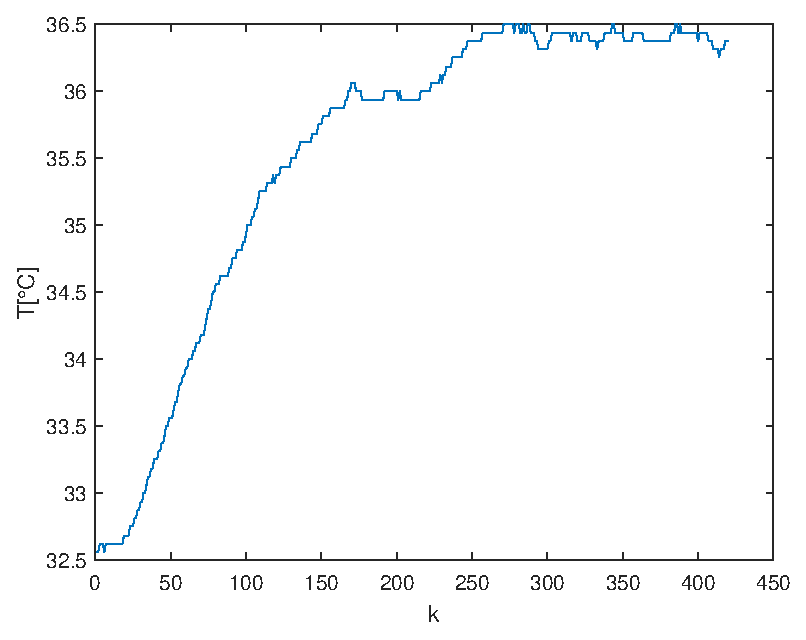
\includegraphics[scale=1]{Rys/Skok20_30.eps}
	\caption{Skok wartości sterowania z 20 do 30}
	\label{skok1}
\end{figure}

\begin{figure}[h!]
	\centering
	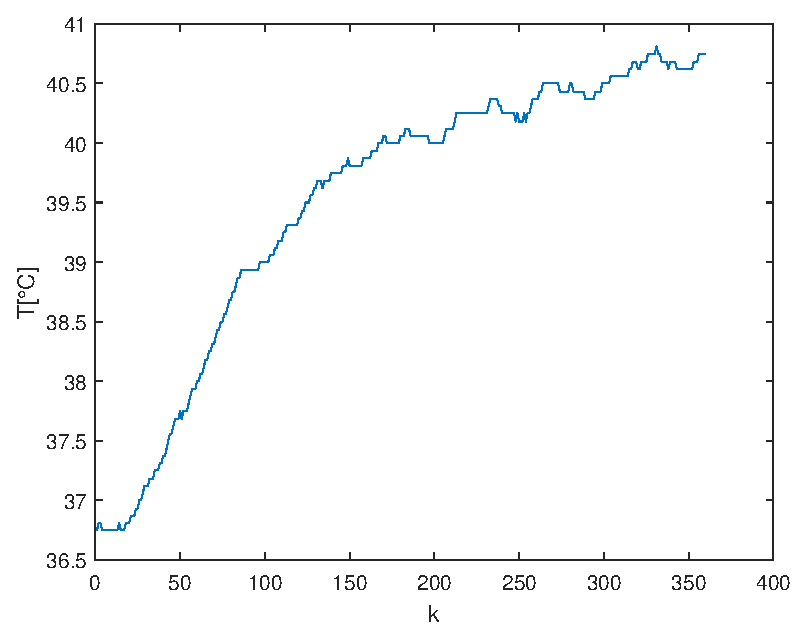
\includegraphics[scale=1]{Rys/Skok30_40.eps}
	\caption{Skok wartości sterowania z 30 do 40}
	\label{skok2}
\end{figure}

\begin{figure}[h!]
	\centering
	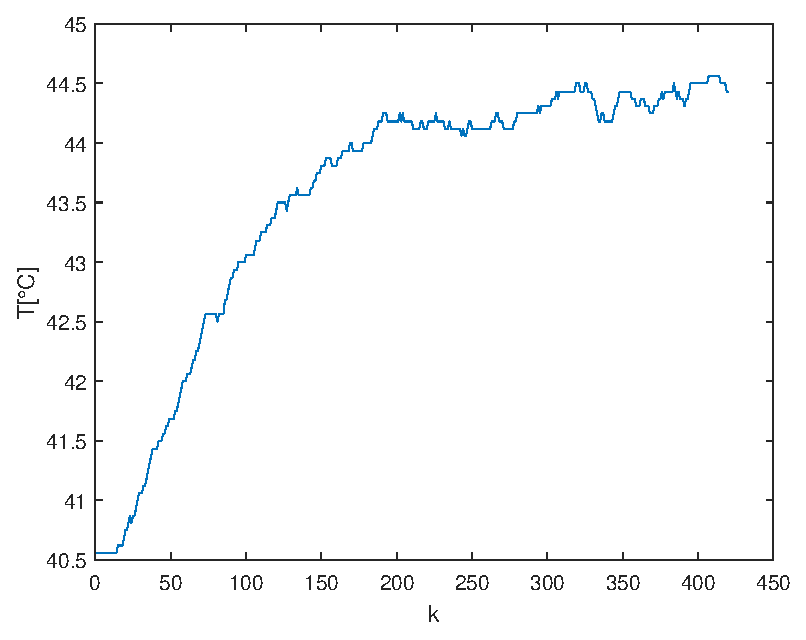
\includegraphics[scale=1]{Rys/Skok40_50.eps}
	\caption{Skok wartości sterowania z 40 do 50}
	\label{skok3}
\end{figure}

\begin{figure}[h!]
	\centering
	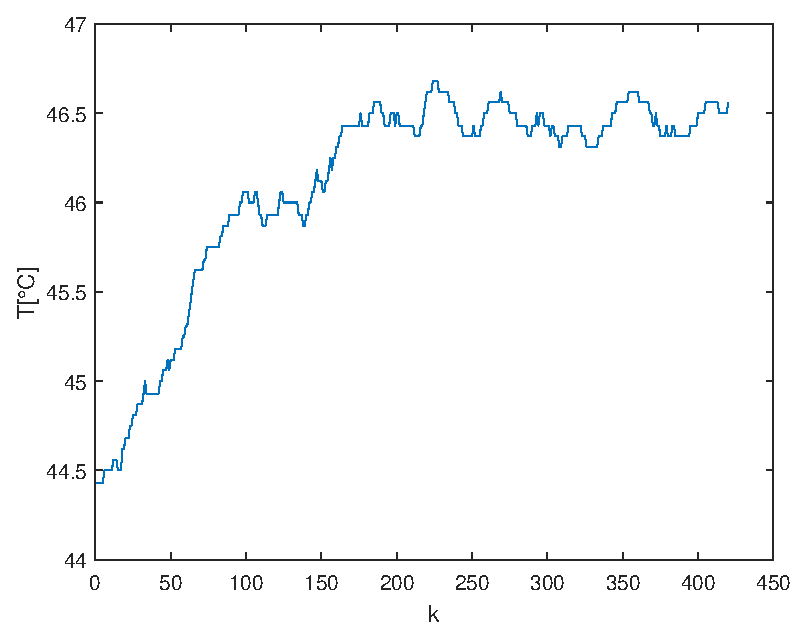
\includegraphics[scale=1]{Rys/Skok50_60.eps}
	\caption{Skok wartości sterowania z 50 do 60}
	\label{skok4}
\end{figure}

\begin{figure}[h!]
	\centering
	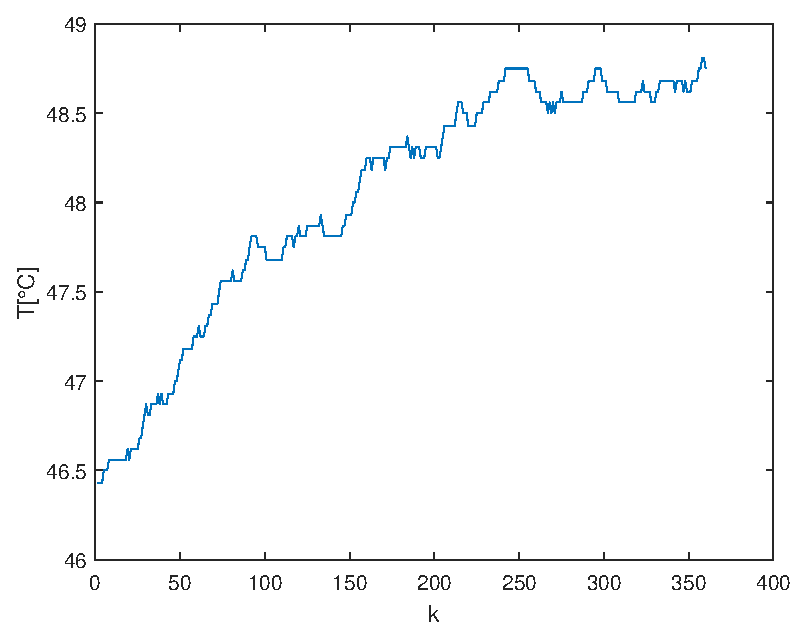
\includegraphics[scale=1]{Rys/Skok60_70.eps}
	\caption{Skok wartości sterowania z 60 do 70}
	\label{skok5}
\end{figure}

\begin{figure}[h!]
	\centering
	\includegraphics[scale=1]{Rys/Skok70_80.eps}
	\caption{Skok wartości sterowania z 70 do 80}
	\label{skok6}
\end{figure}

\FloatBarrier

Wyniki przedstawiono w tabeli:

\begin{center}
 \begin{tabular}{ | m{1cm}| m{1cm} | }
 \hline
 G1[\%] & T[\degree C]   \\
 \hline
 20 & \num{32,43}   \\ 
 \hline
 30 & \num{36,62 }  \\
 \hline
 40 & \num{40,75}  \\
 \hline
 50 & \num{44,31} \\
 \hline
 60 & \num{46,5}  \\ 
 \hline
 70 & \num{48,68}  \\ 
 \hline
 80 & \num{50,56}  \\
 \hline


\end{tabular}
\end{center}


\section{Charakterystyka statyczna obiektu}

Charakterystykę statyczną obiektu w przedziale sterowań G1 od 20 do 80\% przedstawiono na wykresie \ref{stat}:

\begin{figure}[h!]
	\centering
	\includegraphics[scale=1]{Rys/Char_stat.eps}
	\caption{Charakterystyka statyczna obiektu}
	\label{stat}
\end{figure}


\section{Wzmocnienie statyczne}

Z wykresu charakterystyki liniowej można stwierdzić, że obiekt nie jest całkowicie liniowy, występuje załamanie charakterystyki w punkcie U=\num{50}\%. Jednak obiekt jest kawałkami liniowy, przejawia właściwości liniowe w przedziale \num{20}-\num{50}\% oraz inne  właściwości liniowe w przedziale \num{50}-\num{80}\% - na tych odcinkach obiekt zachowuje się praktycznie w sposób liniowy. Dlatego też możemy policzyć wzmocnienie statyczne obiektu w tych przedziałach sterowania:

\begin{equation}
K_{\num{20}-\num{50}\%}= \frac{Y(50)-Y(20)}{50-20}=\frac{44,31-32,43}{50-20}=0,396
\label{zad2_wzm_statyczne_wzor1}
\end{equation}


\begin{equation}
K_{\num{50}-\num{80}\%}= \frac{Y(80)-Y(50)}{80-50}=\frac{50,56-44,31}{80-50}\approx 0,208
\label{zad2_wzm_statyczne_wzor2}
\end{equation}



\chapter{Zastosowanie tradycyjnych regulatorów PID i DMC}




\section{Regulator PID}

\subsection{Postępowanie}

Zarówno w przypadku regulatora PID oraz DMC zostaną użyte skrypty z projektu nr 1 ( \verb|doLabPID.m|  \verb|doLabDMC.m|). Jedyna zmiana nastąpi w wysyłaniu sterowania do obiektu, gdzie funkcję \verb|sendControls| zastępujemy funkcją \verb|sendNonlinearControls|, która ma na celu symulację braku liniowości obiektu na całym obszarze wartości sterowań. 

\subsection{Wyniki symulacji}

Wyniki symulacji przestawiono na wykresie \ref{naiwnyPID}:

\begin{figure}[h!]
	\centering
	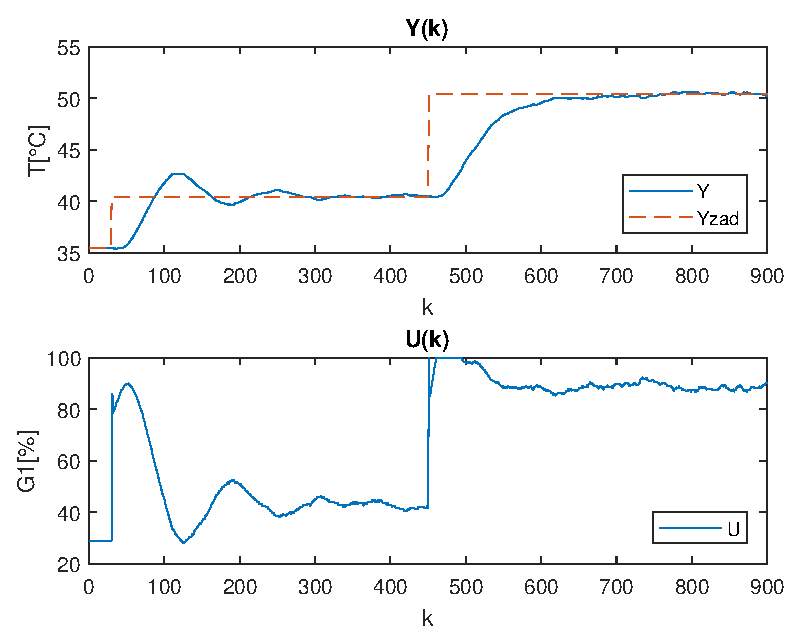
\includegraphics[scale=1]{Rys/NaiwnyPID.eps}
	\caption{Symulacja dla pojedynczego regulatora PID o parametrach $K=9,65, T_{i}=60,  T_{d}=0,17 $}
	\label{naiwnyPID}
\end{figure}


Błąd (suma kwadratów odchyłek) wyniósł E= \num{6077}.

\FloatBarrier

\section{Regulator DMC}

Wyniki symulacji przedstawiono na wykresie \ref{naiwnyDMC}:

\begin{figure}[h!]
	\centering
	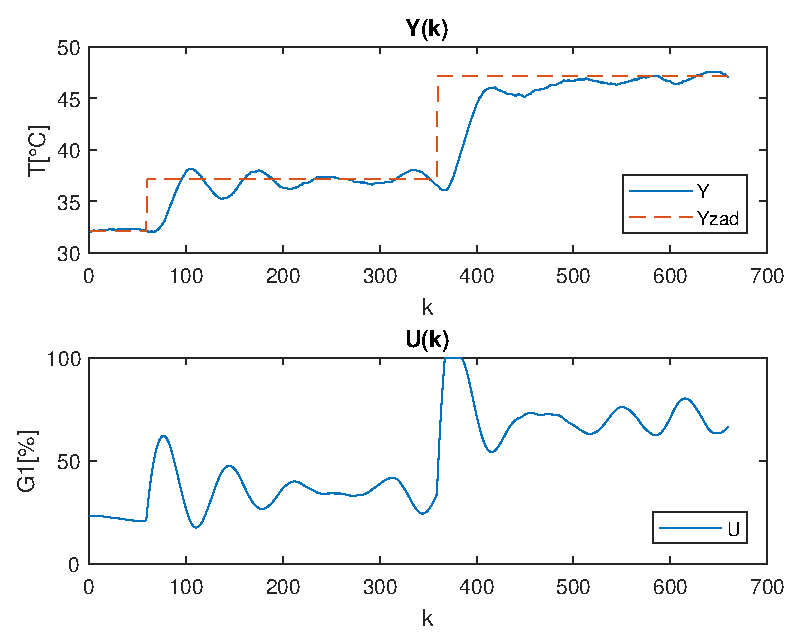
\includegraphics[scale=1]{Rys/NaiwnyDMC.eps}
	\caption{Symulacja dla pojedynczego regulatora DMC o parametrach $D=360, N=120, N_{u}=20, \lambda=1 $}
	\label{naiwnyDMC}
\end{figure}

Błąd (suma kwadratów odchyłek) wyniósł E= \num{3795} (wyniki można ze sobą porównywać mimo krótszego czasu trawnia symulacji, liczba skoków pozostała ta sama - tam są generowane głównie uchyby).

\section{Wnioski}

Pomimo że regulatory działają, temperatura zadana jest mniej więcej osiągana, jednak ich regulacja jest dosyć wolna, a wyjscie oscyluje. W celu poprawy regulacji dokonano rozmycia tych regulatorów.
\chapter{Rozmywanie regulatorów}

\section{Funkcje aktywacji}

Dla obu regulatorów dobrano identyczne funkcje aktywacjii dla trzech regulatorów lokalnych. Rozmywane one są względem wartości sterowana w poprzednim momencie. Zdecydowano się na to z dwóch powodów: po pierwsze układ może zmieniać swoje punkty pracy w zależności od warunków atmosferycznych otoczenia, rozmywanie po wyjściu naraża nas na wpływ takich odchyleń i spadek jakości regulacji; po drugie nieliniowość na obiekcie jest wprowadzana sterowaniem, tzn. obiekt (według tego co ustalono na projektach 1 oraz 2) jest w miarę liniowy, a jego właściwości nie mogły się zmienić, nieliniowość narzucana jest przez funkcję \verb|sendNonlinearControls|, która jakoby przerabia sterowanie tak, aby układ zachowywał się jak nieliniowy. \\

Pierwszy regulator lokalny będzie aktywny głównie w przedziale 0-50\% (na tym przedziale obiekt zachowuje się jak liniowy), drugi w przedziale 45-55\%, a trzeci głównie w przedziale 50-100\%, patrz rysunek \ref{fun_przyn}:

\begin{figure}[h!]
	\centering
	\includegraphics[scale=0.75]{Rys/Przynaleznosc.eps}
	\caption{Funkcje aktywacji regulatorów lokalnych}
	\label{fun_przyn}
\end{figure}

\FloatBarrier

\section {Rozmyty regulator PID}

\subsection{Algorytm}

W celu weryfikacji po

\appendix
\end{document}